\chapter{Related Works} \label{sec:related}
Recently, different algorithms have been proposed to craft 
adversarial attacks against object detection.

Adversarial attacks for object detection are systematically studied for the first time in \cite{xie2017adversarial} with the algorithm DAG. The authors proposed an iterative white-box method that tries to assign adversarial labels to each RoI in the image adding noise to the original image. It runs gradient backpropagation to minimize a loss function computed as the sum, with respect to all the targets in the image, of the differences between the score assigned to the original correct class and the one assigned to the adversarial incorrect class.

Co et al. proposed in \cite{procNoise_co2019} to create attacks to object detection systems by applying procedural noise functions, in particular Perlin noise and Gabor noise, to the original images. They hypothesized that procedural noise, which exhibits patterns visually similar to the Universal Adversarial Perturbations (UAPs) proposed by \cite{MoosaviDezfooli2017UniversalAP}, can also act as UAPs. They empirically demonstrated the vulnerability of some Deep Convolutional Networks to this procedural noise, parameterized by Bayesian Optimization, for the classification task on the ImageNet dataset. Then, they demonstrated that the same procedural noise is able to attack also Yolo v3 object detector on the dataset MS COCO.

In \cite{wang2020adversarial} the authors represented the black-box attack problem as an optimization problem in the manifold of sample images, and then designed a GA-PSO algorithm to solve the problem and generate adversarial examples. In particular they create the image particle swarm with attacking images generated as randomly (heavily) noised version of the original image and then try to optimize their quality moving them towards the original image.

We have to note that all the methods described above share the same general structure: optimized noise added to the original images in order to obtain effective attacks. They differ on the noise applied and on the optimization algorithm used but the high level idea is the same. Moreover, all of them create restricted attacks since they control the modifications on the images by means of $L_p$-norms.  

Our work falls in the same category but with significant differences: we craft the attacks as compositions of Instagram-inspired filters (instead of noise) and we optimize them by means of a nested evolutionary algorithm. This algorithm combines GA (genetic algorithm) to obtain the composition and ES (evolution strategy) to optimized the parameters of the filters. Moreover, we use a multiobjective optimization approach that can take into account different conflicting objectives such as the minimization of mAP or IoU and the maximization of the image quality. The application of non limited filters and the image quality assessment in the multi-objective optimization process allow us to create unrestricted attacks able to produce image artifact-free that appear more natural than the ones produced by the other methods. The differences between attacking images produced applying the procedural noise proposed in \cite{procNoise_co2019} and the ones produced by our algorithm can be observed comparing the images in Figures \ref{fig:objdet_samples}--\ref{fig:procnoise_samples} where examples of attacking images produced by our method (Fig. \ref{fig:objdet_samples}) and procedural Noise method (Fig. \ref{fig:procnoise_samples}) are shown. The patterns produced by procedural noise are evident.

Another class of adversarial attacks to object detection includes the methods that transform white-box attacks into black-box attacks exploiting their transferability across different models. In case of high transferability, white-box  methods can be used in a black-box setting transferring the attacks found for a given known model towards an unknown model. 

In \cite{liang2021parallel} the authors showed that optimizing rectangular perturbations (using a white-box method against a given model) on regions having higher probability to contain objects provides effective attacks to object detection systems that use different DNN as backbone.  

An interesting exception is represented by the \textit{Dispersion Reduction} method proposed in \cite{Lu_2020_CVPR}. The authors' idea is to transfer the concept of image "contrast"  into the feature maps produced by a convolutional neural networks. As lowering the contrast of an image can make the objects depicted unrecognizable, they proposed to reduce the contrast of an internal feature map to degrade the object detection. They formally defined the problem as a minimization problem of the dispersion (they use standard deviation) of the intermediate feature map of the modified image constrained by the $L_\infty$-norm with respect the original one.

\chapter{The Algorithm} \label{sec:algorithm}

In this thesis we extend the AGV method previously proposed in \cite{AGV-evoapps,AGV-wiiat} to craft adversarial attacks against methods for object detection. The core algorithm is structured as a nested-evolutionary algorithm which finds an optimal unrestricted adversarial perturbation by composing and optimizing multiple image filters. The algorithm consists of two optimization steps: given a predefined set of popular image filters, the outer optimization phase focuses on finding a sequence of filters to apply to the image, while the inner step optimizes the parameters of these filters to obtain the attack. The core algorithm is described in Algorithm \ref{agv_core} and details on the algorithm components are provided in the next sections.

%\noindent The structure of the core algorithm is reported in Algorithm 1.
% \begin{figure}[h] \label{fig:AGV_alg}
% \centering
% \includegraphics[width=0.7\textwidth]{agv_core_algorithm.PNG}
% \caption{AGV core algorithm}
% \end{figure}

\begin{figure}[]
\centering
    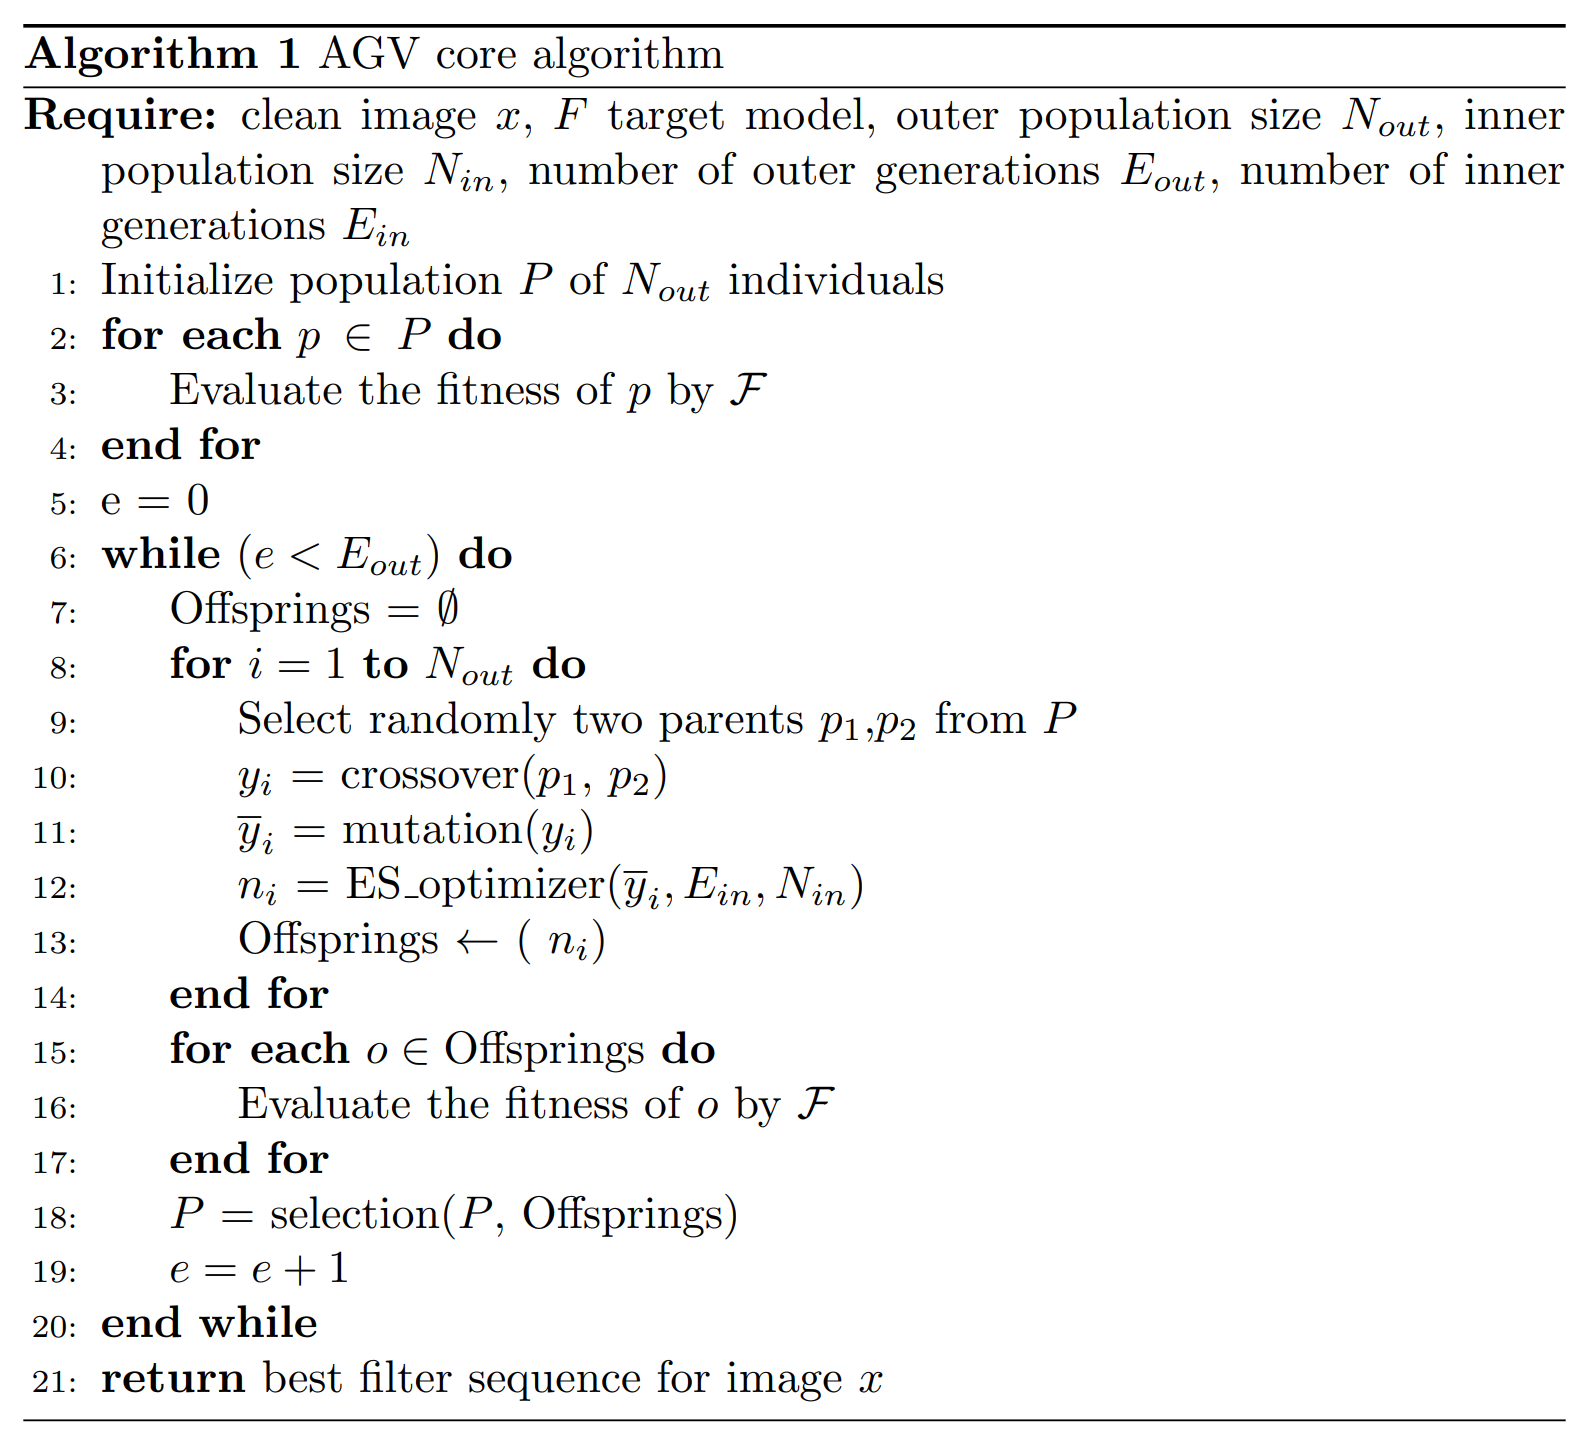
\includegraphics[width=1.0\textwidth]{Attack/charts/agv_alg.png}
    \caption{}
    \label{agv_core}
     
      %\caption{Normal Case: 1 Request \& 1 Response.}
\end{figure}

\section{General Problem Definition}
Given a set $S = \{ f_1, f_2, \dots, f_m \}$ of Instagram inspired image filters, and a clean image $x$, we want to find a sequence of $n$ parametrized filters $\{f_{k_1}(\alpha_1,s_1),\ldots,f_{k_n}(\alpha_n,s_n)\}$ able to produce an adversarial attack against the victim model $F$ such that 
 \begin{equation}      
 \begin{array}{cc}
      x^* = f_{k_n}(\alpha_n,s_n)(\dots f_{k_2}(\alpha_2,s_2)(f_{k_1}(\alpha_1,s_1)(x)))\\
      x^* = \mathrm{argmin} \; ODP(F(x^*))
      
 \end{array}
    \label{eq:filter_application}
 \end{equation}
 where $ODP$ is a measure of the Object Detection
Performance.
Specific definition of $ODP$ is provided in the following Sections \ref{sec:objdet}.
 

\section{Image Filters}

The unrestricted adversarial perturbation is inspired by the popularity of Instagram filters and their ease of use. In particular, commonly-used well-known image filters are employed in order to alter  different features of an image, such as contrast, saturation, brightness, etc. Such image manipulations are able to generate a variety of editing styles, ranging from more vivid and bright colors to more soft and warm looks. The implemented filters are Clarendon, Juno, Reyes, Gingham, Lark, Hudson, Slumber, Stinson,
Rise, and Perpetua.
Each filter modifies an image with respect to different aspects and each filter is parameterized by two main parameters that the inner algorithm has to optimize: intensity $\alpha$ and strength $S$.

The parameter $\alpha$ controls the level of intensity of each basic feature of the filter implementation, like saturation, brightness, contrast, gamma correction and so on. On the other hand, we define the parameter $s$ as the parameter of the convex interpolation between the original image $x$ and the its filtered version $x^*$ that allows us to control the strength of the filter application.
\begin{equation}
strength(x,x^*,s) = (1.0-s) \cdot x + s \cdot x^*
\end{equation}

where in the case of $s=0$ the image remains unaltered, while with $s=1$ the filter function applies the maximum allowed manipulation and returns the filtered image $x^*$.\\

\noindent \textbf{Image Quality Assessment}: Heavy applications of multiple filters can create unnatural looking images which cannot bypass a human judgement. Therefore, in order to keep the aesthetics, naturalness and distortions within acceptable parameters, we employ the \textit{Structural Similarity Index Measure} (SSIM), that is a method for predicting the perceived quality an image. SSIM, introduced by Wang et al. \cite{SSIM}, is a well-performing and widespread Full-Reference method (meaning that it requires a reference image to compute the quality score) that is able to automatically evaluate the quality of the adversarial examples generated by the algorithm. SSIM is a context-aware metric that measures the image degradation as perceived changes in the structural information. Structural information represents the structure of objects in an image which are independent of contrast and luminance. Therefore, SSIM is defined as a comparison function of contrast, luminance and structure computed over the image. By design, the metric satisfies the symmetry, boundedness and unique maximum property that assures an upper value of 1 if and only if the two images compared are identical. In practice, a score higher than 0.99 indicates that the images are indistinguishable. 



\section{Outer optimization}
We employ a genetic algorithm for the outer optimization step where a population of $N$ candidate filter combinations is evolved towards an optimal solution.
%A new generation is created by altering and mutating 
%The genetic operators are applied in order to breed a new generation: 
To create a new generation, randomly selected individuals are altered and mutated by means of the genetic operators, such as crossover and mutation. Then, a problem-specific fitness function is used to measure the quality of each candidate and only the $N$ fittest solutions are selected and passed onto the next generation.

%\noindent The main algorithmic steps are the following:
\begin{itemize}
    \item {\bf Initial Population}: each individual is generated by randomly choosing a predefined number of filters with both parameters set to 1. 
    \item { \bf Crossover}: the generation of new off-springs is handled by a standard one-point crossover operation where the genetic information from 
    a pair of randomly selected candidates is combined in order to produce a new solution. Thus, the off-spring will share genetic characteristics with both parents along with their optimized parameters.
    \item {\bf Mutation}: is applied in order to maintain genetic diversity from one generation to another. It consists of replacing a filter from a sequence with another one based on a probability mutation. Moreover, in this case, the substituent filter is initialized with random parameter values in order to perform mutation over the parameters as well.
    \item {\bf Selection}: at the end of each generation, a fitness-based selection process is used to pick the $N$ fittest individuals from the set composed of parents and off-springs having size $2N$. 
    %The above mention steps (with except of initialization) are repeated  until a termination criteria is met, i.e. the algorithm reaches the allowed number of generations. 
    In particular, since one of the aims of this work is to create natural looking, artifacts free adversarial samples, we incorporate into the selection process both a measure of the attacking ability and an image quality metric. Therefore, the selection process is defined as a multi-objective optimization problem where we want to minimize the performance on the task  \textit{Object Detection Performance (ODP)}  while $SSIM(x, x^*)$  is maximized. Thus, the multi-objective fitness function to minimize is formulated as:
    \begin{equation} \label{eq:general_fitness}
       \mathcal{F}(x,x^*) = \{ ODP(x^*), 1-SSIM(x, x^*)\},
    \end{equation}
    where $x$ is the original image, $x^*$ is the modified image according to (\ref{eq:filter_application}), 

 and $SSIM$ is the metric used to control the applied perturbation. The multi-objective problem is handled by the non dominated sorting and crowding distance NSGA-II algorithm \cite{NSGA-II}.
\end{itemize}

\section{Inner optimization}

The parameter optimization is managed by means of $(1,\lambda) $ Evolutionary Strategy.
In particular, this algorithm evolves a population of lists of parameters for every individual in the outer algorithm. For each inner individual batch, $\lambda$ samples are created by perturbing the original individual. ES uses the fitness values of the batch samples  to estimate a gradient towards a better solution.  The gradient value is then used to update the original individual. This  process is performed over multiple iterations. 

\section{Allowed Queries}
An important aspect that has to be taken into account 
for real-world attacks is the amount of queries to the victim model that are necessary to craft effective attacks.
This is important because it is strictly related to the possibility of being intercepted by defense mechanisms that can be implemented to protect the victim model.

Our algorithm works with limited accesses to the victim model that is called every time we have to compute the fitness function. Besides the explicit calls to the evaluation function made in the initialization step and in the last step of each outer iteration, we have to consider the $E_{in}\times N_{in} $ calls made by the inner optimization phase (filters' parameters optimization) for each element in the outer population. 
Hence, the maximum number of allowed queries can be easily computed as: 
\begin{equation} \label{eq:queries}
   Q_{MAX} =  N_{out} + E_{out} \times ( N_{out} \times  E_{in} \times N_{in} + N_{out}),
\end{equation}
where $N_{out}$ is the size of the outer population, $N_{in}$ is the size of the inner population, $E_{out}$  is the number of outer generations, and $E_{in}$ is the  number of inner generations.





\section{AGV Attacks on Object Detection} \label{sec:objdet} 
%punti di differenza rispetto all'alg originale
In order to apply AGV algorithm to Object Detection we have to define the fitness function used by the algorithm to guide the search.
The fitness function for Object Detection uses, besides SSIM as described in (\ref{eq:general_fitness}), the function ODP (Object Detection Performance) as implementation of Task Performance function, hence
$$\mathcal{F}(x,x^*) = \{ ODP(x,x^*), 1-SSIM(x, x^*)\}$$
%TP evaluates the performance of the model on a given image (X) in which we applied the proposed filters (Xf). This is done to approximate the optimal ones and their parameters in order to minimize the performance of the model in X.

To compute $ODP$, we paired each bounding-box detected in the original image $x$, i.e. each $b_i$ in $F(x)$, with ones detected in the perturbed image $x^*$, i.e. $b^*_i$ in $F(x^*)$, having the same label $c^*_1=c_i$ and $IoU> 0.5$.
For each pair, ODP is increased by $IoU(b_i,b^*_i)/\vert F(x)\vert$, so that the performance is the weighed sum of the $IoU$ of the paired boxes with respect the total number of boxes in the original image.
Minimizing this function allows us to fool the model into getting the wrong classification (raise the misclassification rate) and to lower the $IoU$ values below the threshold. The algorithm is proposed  in Algorithm \ref{algODP}.



\begin{figure}[ht]
\centering
    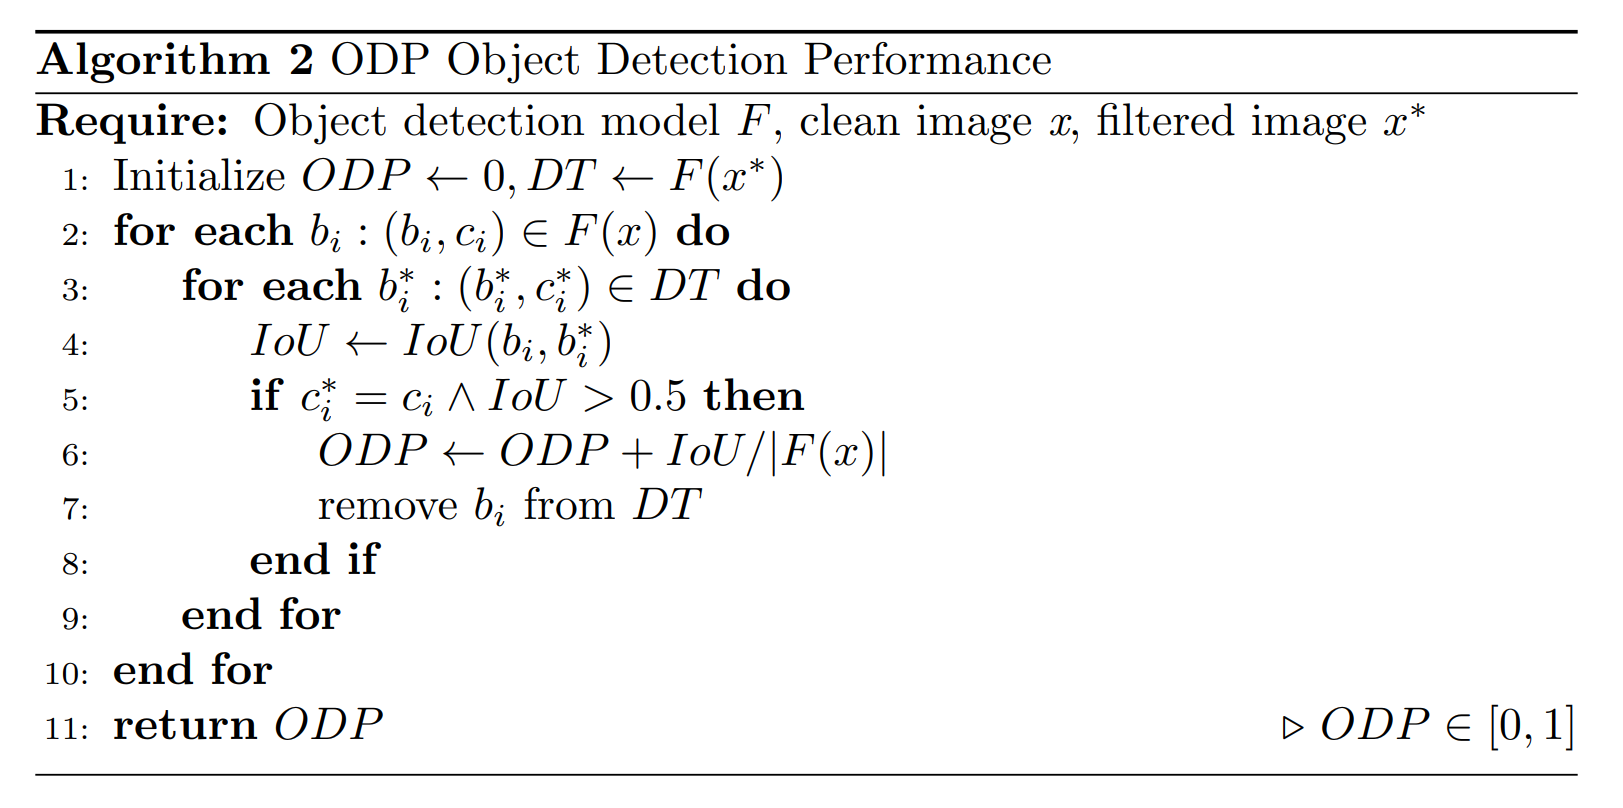
\includegraphics[width=1.0\textwidth]{Attack/charts/odp_alg.png}
    \caption{}
    \label{algODP}
     
      %\caption{Normal Case: 1 Request \& 1 Response.}
\end{figure}

% Given $Xf$ an image derived from the clean one by applying a sequence of filters, $Y$ the bounding-boxes predicted by the model on the clean image $X$, the Object Detection Performance (ODP) function is evaluated by the following:
% \begin{equation}
% %\begin{aligned}
% %\resizebox{.8\hsize}{!}{
%     ODP(Xf,Y)=\sum_{i=1}^{len_y} 1/len_y \sum_{j=1}^{len_x} IOU(y\_bbox_i,x\_bbox_j)      [label(y\_bbox_i)=label(x\_bbox_j) \wedge IOU(y\_bbox_i,x\_bbox_j)]
% %\end{aligned}
% %\normalize
% \end{equation}
% with $y\_bbox \in Y$ and $x\_bbox \in model.predict(Xf)$.
